                                       

An Real Time Operating System (RTOS), is an operating system must be able to
deal with a time and event sensitive activities. The RTOS is intended intended
to be \textit{predictable} and \textit{determinant}\cite{RTOSMantis}. These
systems are also designed to limit the amount of over head that is required to
context switch between tasks. This is done my making many critical decisions
prior to runtime.



\subsection{Tasks}

There are three different types of tasks in the RTOS; system tasks, periodic tasks and round robin tasks. These tasks are ordered in decreasing priority levels.

\begin{description}
    \item[System Tasks]
    System tasks are of the highest priority task. If a system task is
    scheduled to run, it will preempt any other task.

    \item[Periodic Tasks]
    Periodic tasks are the next level below system tasks---middle priority.
    These tasks are scheduled to run periodically based on time (clock cycles).
    Periodic tasks are declared at the beginning of the program. A \texttt{PPP}
    array is also declared. This array allots time to each task and also
    declares an order for the periodic tasks. A periodic task is not allowed to
    take more time than has been allotted.  If this occurs, it is called a
    timing violation, and the system halts.

    \item[Round Robin Tasks]
    The final level---low priority -- are the round robin tasks. Round robin tasks
    are executed in the \textit{idle} time between periodic tasks.The kernel
    maintains a FIFO queue containing all of the round robin tasks. On each clock
    cycle, if the system is not attending to either a System or Periodic task then
    the next RR tasks is removed from the queue and is run for exactly one tick
    after which it is returned to the end of the FIFO queue. On the next cycle, if
    the higher priority tasks have not regained control, then the proceeding RR
    task is removed from the queue.  
\end{description}



\subsection{Events and Timeouts}

System and round robin tasks are capable of waiting for an event a timeout, or
either. The reason that only system and round robin tasks are allowed to wain on events, is that if a periodic task waits longer than its time allowance a timing violation would occur. \\

\noindent{\bf Events}\\
Events are initiated at the beginning of the program. Tasks that wait for an event are placed on a queue. The first item in the queue will continue when another task \textit{signals} that event. All of the elements will be released from the queue if another task \textit{broadcasts} that event. \\

\noindent{\bf Timeouts}\\
The kernel maintains a variable \textit{now} indicating how many ticks have occured since program instantiation. When a task waits a certain amount of time, it will return normal operation after n ticks have passed.





The RTOS used for this project was created by Scott Craig and Justin Tanner \cite{RTOSSJ}. This RTOS is written in a mixture of C and assembly and is primarily written to support periodic tasks.   




\noindent\textbf{Sonar}

The integration of the sonar and the RTOS is based on the report by Will
Logan, Cambria Hanson and Jason Kereluk \cite{autoB}.

-Overall Design of our RTOS
-GANT charts
-Timming Diagrams
-Code

\subsection{Tasks for Hovercraft 1---The leader}
In this project, hovercraft 1 assumes the role of a leader. It will navigate the
environment and make decisions to traverse the environment. Those decisions are,
then, relay to the trailing hovercraft, hovercraft 2. As a result, the
implementation hovercraft 1 is quite complex. This section will explain the
breakdown of the tasks in the implementation of hovercraft 1.

\begin{lstlisting}[float=th,label=lst:h1ppp,
                   caption={\texttt{PPP} array for hovercraft 1}]
const unsigned char PPP[] = {FIRE, 4, LISTEN, 1, FIRE, 4, LISTEN, 1, FIRE, 4, LISTEN, 1, MOTOR, 5};
\end{lstlisting}
The \texttt{PPP} array of hovercraft 1 is shown in listing \ref{lst:h1ppp}.
There are in total seven tasks, and the first six tasks triggering and listening
to the three sonars. In listing \ref{lst:h1sonarfire}, the implementation of the
\texttt{FIRE} task uses the built-in \texttt{Task\_Next()} function to trigger
the three sonars one by one. First, the task will trigger the front sonar, then
it will give up the CPU and allows the listen task (as shown in listing
\ref{lst:h1sonarlisten}) to calculate the distance. When the distances are
stored in their respective variables, the \texttt{MOTOR} task will run. Within
the \texttt{MOTOR} task, it will decide what speed the two motors should spin.
The code for the \texttt{MOTOR} is shown in listing \ref{lst:h1motor}.

\begin{lstlisting}[float=thp,label=lst:h1sonarfire,
                   caption={\texttt{FIRE} Task}]
void fire_sonar(void) {
	for(;;) {
		trigger_sonar(FRONT);
		Task_Next();
		trigger_sonar(RIGHT);
		Task_Next();
		trigger_sonar(LEFT);
		Task_Next();
	}
}
\end{lstlisting}

\begin{lstlisting}[label=lst:h1sonarlisten,float=tbh,
                   caption={\texttt{LISTEN} Task}]
void listen_sonar(void) {
	for(;;)	{
	    s_forward= read_distance();
	    Task_Next();
	    s_right = read_distance();
	    Task_Next();
	    s_left = read_distance();
	    Task_Next();
	}
}
\end{lstlisting}

\begin{lstlisting}[label=lst:h1motor,float=th,
                   caption={\texttt{MOTOR} Task}]
void motor_task(void) {
	for(;;) {
    	if(s_front < MIN_DISTANCE &&  s_left >MAX_DISTANCE) {
            r_dir= FORWARD;
            r_duty = 255;
            l_dir = BACKWARD;
            l_duty = 255;
   		} else if (s_front < MIN_DISTANCE && s_right>MAX_DISTANCE) {
            r_dir = BACKWARD;
            r_duty = 255;
            l_dir= FORWARD;
            l_duty = 255;					
    	} else if (s_left < MIN_DISTANCE && s_right > MAX_DISTNACE) {
            l_dir = FORWARD;
            l_duty = 255;
            r_duty = 0;
   	 	} else if (s_right<MIN_DISTANCE && s_left > MAX_DISTANCE) {
            r_dir = BACKWARD;
            r_duty = 255;
            l_duty = 0;
    	} else {
            Signal_Event(stop);
    	}
        setMotorDirection(&rightMotor,r_dir;
        setMotorDuty(&rightMotor, r_duty);
        setMotorDirection(&leftMotor,l_dir);
        setMotorDuty(&leftMotor, l_duty);
	}
}
\end{lstlisting}

\begin{minipage}{6.5in}
        \centering
        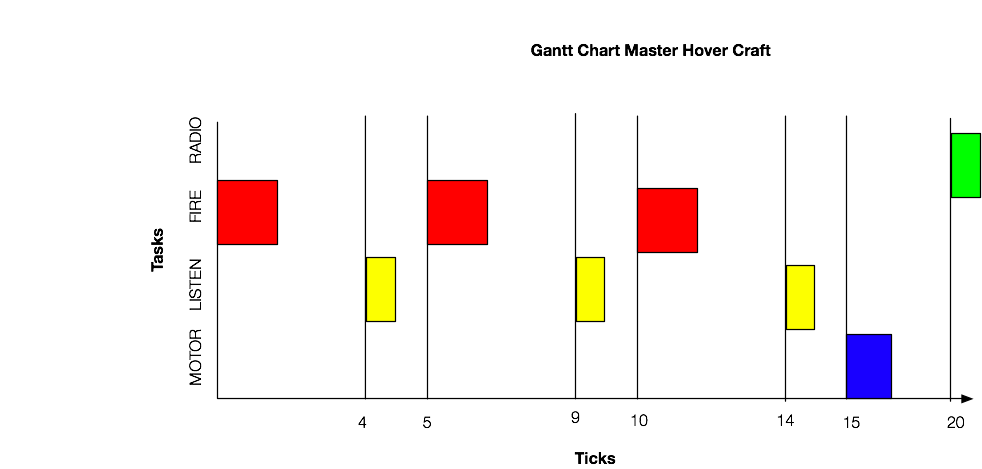
\includegraphics[width = 100mm]{imageSources/Gantt.png}
        \captionof{figure}{Gantt chart for the master hovercraft}
        \label{gantt}
\end{minipage}
